\documentclass[xcolor=svgnames]{beamer}
% \usetheme{JuanLesPins}
\usetheme{CambridgeUS}
\usecolortheme{crane}
\usepackage{fontenc}

\usepackage[english]{babel}
\usepackage[latin1]{inputenc}
\usepackage{times}
\usepackage[T1]{fontenc}
\usepackage{fontenc}
\usepackage{amssymb}
\usepackage{multicol}
\usepackage{multirow}

\usepackage{amsmath,amssymb}
\usepackage{tikz}
\usepackage{verbatim}
\usepackage{subfigure}
\usetikzlibrary{arrows,shapes,positioning,backgrounds}
\usetikzlibrary{patterns}


\usepackage{times}
\usepackage{colortbl}
\usepackage{color}

\usepackage{tocvsec2}
\setlength{\leftmargini}   {13pt} 
\setlength{\leftmarginii}  {13pt} 
\setlength{\leftmarginiii} {13pt} 


\title[TT en Dise�o de Sistemas Embebidos]{TRANSFERENCIA TECNOL�GICA Y DE CONOCIMIENTOS EN EL DISE�O DE SISTEMAS EMBEBIDOS}
% \author{Carlos Iv�n Camargo Bare�o\\
%         Director: Luis Fernando Ni�o (PhD)
%         }

\author[Carlos Camargo]{Carlos Iv�n Camargo Bare�o\inst{1}  \\ \and Director: Luis Fernando Ni�o\inst{2}}
\institute[UNAL]{

\inst{1}Departamento de Ingenier�a El�ctrica y Electr�nica \and
\inst{2}Departamento de Ingenier�a de Sistemas e Industrial}

\pgfdeclareimage[height=.5cm]{logo}{../images/logo_unal}
\logo{\pgfuseimage{logo}}


\usepackage{etoolbox}
\makeatletter
\patchcmd{\@makefntext}{\insertfootnotetext{#1}}{\insertfootnotetext{\tiny#1}}{}{}
\makeatother


\begin{document}

\begin{frame}
\frametitle{}

\setbeamertemplate{background canvas}[vertical shading][bottom=blue,top=structure.fg!25]
\setbeamertemplate{background}{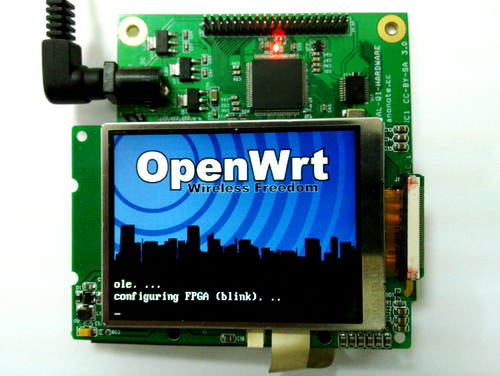
\includegraphics[width=\paperwidth] {../images/SAKC_LCD.png}}


\begin{figure}[htpb]
    \begin{center}
        \newcommand{\daywidth}{2.2 cm}

        \begin{tikzpicture}[x=4cm, node distance=0 cm]
        \tikzstyle{day}=[draw, rectangle,  minimum height=0.5cm, minimum width=\daywidth, fill=yellow!20,anchor=south west]
        \tikzstyle{hour}=[draw, rectangle, minimum height=.5 cm, minimum width=2cm, fill=blue!30,anchor=north east]

        % Styles for events
        \tikzstyle{hours}=[rectangle,draw, minimum width=\daywidth, anchor=north west,text centered,text width=4 em]
        \tikzstyle{1hour}=[draw, rectangle,  minimum height=0.5cm, minimum width=4cm, fill=blue!20,anchor=south west]
        \tikzstyle{2hours}=[hours,minimum height=2cm]
        \tikzstyle{4days}=[draw, rectangle,  minimum height=0.5cm, minimum width=4.4cm, fill=yellow!20,anchor=south west]
        %Style for type of sequence 
        \tikzstyle{Private} = [2hours,fill=red!20]
        \tikzstyle{Club}    = [2hours,fill=green!20]
        \tikzstyle{Common}  = [2hours,fill=blue!20]
        \tikzstyle{Public}  = [2hours,fill=brown!20]
        %Position of sequences
        \node[hour, rotate=90] (8-9)   at (1,1)   {Exc.};
        \node[hour, rotate=90] (9-10)  [left = of 8-9] {No exc.};
        \node[Private] (Private) [right = 0cm of 8-9.south] {Privado}; \node[Club]   (Club)   [right = of Private] {Club};
        \node[Common]  (Common)  [below = of Private]       {Com�n};  \node[Public] (Public) [right = of Common]  {P�blico};

        % % Positioning labels

        \node[day] (lundi) [above = of Private] {Rival};
        \node[day] (mardi) [right = of lundi]   {No rival};

        \node[4days] (Rivality) [above = 0cm of lundi.north east] {Rivalidad};
        \node[1hour, rotate=90] (Excludability) [above = 0cm of 8-9.north west] {Exclusi�n}; 
        \end{tikzpicture}
    \end{center}
  \caption{Clasificaci�n general de los bienes. fuente: \cite{CMS06}} 
  \label{goods_class}
\end{figure}




\end{frame}
% 
% 
% \frame{}
%   \movie[height=1.25in, width=1.5in, poster]{}{xxxx.mov}
\end{document}